% IOE MSC Latex Template by
% Santosh Giri, Assistant Professor, DOECE, Pulchowk Campus, IOE, TU
\documentclass[12pt]{report}
\usepackage{xcolor}
\usepackage[utf8]{inputenc}
\usepackage{natbib}%referencing
\usepackage[left=1.0in,right=1.0in,top=.8in,bottom=.8in]{geometry}
\usepackage{float}
\linespread{1.3}
\usepackage{graphicx}%figures
\usepackage{rotating}%landscape
\usepackage{amsmath}%math
\usepackage{longtable}
\usepackage{array}
\usepackage{booktabs}
\usepackage{tabularx}
\usepackage{tikz}
\usepackage{pgfgantt}
\usetikzlibrary{shapes.geometric, arrows.meta, positioning}

\usepackage{titlesec} %formatting chapters
%\titlespacing*{<command>}{<left>}{<before-sep>}{<after-sep>}
\titlespacing*{\chapter}{-15pt}{10pt}{15pt}
\titlespacing*{\section}{0pt}{0pt}{5pt}
\titlespacing*{\subsection}{0pt}{5pt}{5pt}
\titleformat{\chapter}[hang]
{\normalfont\huge\bfseries}{\chaptertitlename\ \thechapter.}{1em}{}
\renewcommand{\chaptername}{}
\graphicspath{{Images/}}%image folder name
%Cover page contents
\title{
\includegraphics[scale=.3]{logotu.jpg}\\
\uppercase\large{
\vspace{.8cm}
    {Tribhuvan University}\\
    {Institute of Engineering}\\
    {Pashchimanchal Campus}\\
    \vspace{.8cm}
    {A Project Proposal On\\COMPARATIVE ANALYSIS OF LoRA-BASED FINE-TUNING OF
mT5-base AND mBART-large-50 FOR NEPALI ABSTRACTIVE TEXT SUMMARIZATION}\\
    \vspace{.8cm}
    {\textbf{Submitted By:}\\Binay Raj Parajuli\\(PAS081MScmk004)}\\
    \vspace{.8cm}
    {\textbf{Submitted To:}\\ Department of Electronics \& Computer engineering}\\
                }
    }
\date{\today} %{Month Year}
\renewcommand{\contentsname}{Table of Contents}

\begin{document}
\maketitle
\pagenumbering{roman}
\setcounter{page}{2} 
%new chapter
% \chapter*{Acknowledgments}
% \addcontentsline{toc}{chapter}{\numberline{}Acknowledgements}
% \\
% Limited to one page only
% \vspace{50pt}\\
% \textbf{Binay Raj Parajuli ( PAS081MSCmk004)}\\
\tableofcontents
\addcontentsline{toc}{chapter}{\numberline{}Table of Contents}
\listoffigures
\addcontentsline{toc}{chapter}{\numberline{}List of Figures}
\listoftables
\addcontentsline{toc}{chapter}{\numberline{}List of Tables}


\chapter{Introduction}
\pagenumbering{arabic}%start Arabic numbering(1,2,3..) from here



\section{Background}
The rapid growth of digital news portals such as Onlinekhabar, Ratopati, Setopati, and Kantipur has produced an enormous volume of Nepali-language text every day. Readers increasingly struggle to keep pace with this information, which makes automatic text summarization a valuable tool for condensing long articles into short, informative summaries while preserving their essential meaning.

Text summarization is broadly divided into two paradigms. \textit{Extractive} summarization selects and stitches together salient sentences directly from the source, whereas \textit{abstractive} summarization generates new sentences that paraphrase and compress the original content, much like a human writer would \cite{lewis2020bart}. Abstractive summarization is generally more fluent and concise but is also more challenging, as it requires the model to genuinely understand and reformulate the source text.

Sequence-to-sequence transformer models have driven remarkable progress in abstractive summarization for high-resource languages such as English \cite{vaswani2017attention, raffel2020exploring}. However, Nepali remains a low-resource language: it is written in the Devanagari script, has rich morphology and complex grammar, and offers only a limited amount of labelled summarization data. Training a large model from scratch under these conditions is impractical.

Multilingual pretrained models offer a compelling alternative. Models such as mT5 \cite{xue2021mt5} and mBART-50 \cite{tang2020multilingual, liu2020multilingual} are pretrained on dozens of languages, including Nepali, and can be adapted to a target task through fine-tuning on a comparatively small dataset. This transfer-learning capability makes them well-suited for Nepali summarization. However, fully fine-tuning such large models updates hundreds of millions of parameters and demands substantial GPU memory and compute, which is often impractical in resource-constrained settings. Parameter-efficient fine-tuning (PEFT) techniques address this by adapting only a small number of additional parameters while keeping the pretrained weights frozen. Among these, Low-Rank Adaptation (LoRA) \cite{hu2021lora} injects trainable low-rank matrices into the attention layers, dramatically reducing the number of trainable parameters and the memory footprint while retaining competitive performance.

This proposal therefore focuses on adapting and comparing two such models mT5-base and mBART-large-50 for Nepali abstractive text summarization using LoRA, training on the Nepali portion of the XL-Sum dataset \cite{hasan2021xlsum} and evaluating the generated summaries with the ROUGE \cite{lin2004rouge} and BERTScore \cite{zhang2020bertscore} metrics.


\section{Problem Statement}
Most abstractive summarization research targets high-resource languages, leaving Nepali comparatively underexplored. The scarcity of large annotated Nepali summarization corpora, together with the language's morphological richness and script-specific tokenization challenges, makes it difficult to build effective summarizers. Moreover, fully fine-tuning large multilingual transformers is computationally expensive and memory-intensive, which is a significant barrier in low-resource and limited-hardware settings. It also remains unclear which class of multilingual model adapts better to Nepali under parameter-efficient fine-tuning: a compact text-to-text model such as mT5-base, or a larger denoising autoencoder such as mBART-large-50. This proposal addresses these gaps by fine-tuning both models with LoRA under an identical pipeline and comparing the quality of the resulting summaries.


\section{Research Questions}
This proposal is guided by the following research questions:
\begin{itemize}
    \item How effectively can mT5-base and mBART-large-50 be fine-tuned for Nepali abstractive text summarization using LoRA?
    \item Which of the two LoRA-adapted models produces more accurate and semantically faithful summaries for Nepali news articles, and at what computational cost?
    \item How do lexical-overlap metrics (ROUGE) and semantic-similarity metrics (BERTScore) compare when used to evaluate the generated Nepali summaries?
\end{itemize}


\section{Research Objectives}
The main aim of this proposal is to develop and comparatively evaluate abstractive summarization models for Nepali by adapting two multilingual transformers using LoRA-based parameter-efficient fine-tuning. The specific objectives are:
\begin{itemize}
    \item To fine-tune mT5-base and mBART-large-50 for Nepali abstractive text summarization using LoRA.
    \item To generate summaries for unseen Nepali news articles using both fine-tuned models.
    \item To evaluate the quality of the generated summaries using ROUGE and BERTScore.
    \item To compare the two models and analyze the effectiveness of LoRA-based fine-tuning for adapting large multilingual models to a low-resource summarization task.
\end{itemize}


\section{Scope and Limitations}
This proposal focuses on supervised abstractive text summarization for Nepali using LoRA-based parameter-efficient fine-tuning of mT5-base and mBART-large-50. Both models are trained and evaluated on the same XL-Sum Nepali dataset using an identical preprocessing pipeline, training configuration, and evaluation metrics (ROUGE and BERTScore) to ensure a fair and reproducible comparison. The work is limited to the Nepali news domain represented in the XL-Sum dataset and does not cover extractive summarization, full fine-tuning, other Nepali domains, or additional model families.


\chapter{Literature Review}
\begin{table}[htbp]
\centering
\footnotesize
\caption{Comparison of Related Studies with the Proposed Research}
\label{tab:literature_comparison}
\renewcommand{\arraystretch}{1.3}

\begin{tabularx}{\textwidth}{|p{2.3cm}|p{2.0cm}|p{2.6cm}|p{1.6cm}|X|}
\hline
\textbf{Reference / Study} &
\textbf{Focus / Domain} &
\textbf{Methodology / Models} &
\textbf{Language} &
\textbf{Relevance to Proposed Research} \\
\hline

Hasan et al. (2021) &
Multilingual Summarization &
mT5 fine-tuned on XL-Sum &
44 languages (incl. Nepali) &
Provides the benchmark dataset and a baseline mT5 model that this work adapts using LoRA. \\
\hline

Xue et al. (2021) &
Multilingual Text-to-Text &
mT5 (mC4 pretraining) &
101 languages &
Introduces one of the two candidate models (mT5-base) adapted in this study. \\
\hline

Tang et al. (2020) &
Multilingual Generation &
mBART-50 &
50 languages &
Introduces the second candidate model (mBART-large-50) for this comparison. \\
\hline

Hu et al. (2021) &
Parameter-Efficient Fine-Tuning &
LoRA (low-rank adapters) &
Model-agnostic &
Introduces the LoRA technique used to fine-tune both candidate models efficiently. \\
\hline

Lewis et al. (2020) &
Abstractive Summarization &
BART (denoising seq2seq) &
English &
Establishes the denoising seq2seq paradigm underlying mBART. \\
\hline

Raffel et al. (2020) &
Transfer Learning &
T5 (text-to-text) &
English &
Establishes the text-to-text framework underlying mT5. \\
\hline

Zhang et al. (2020) &
Evaluation Metric &
BERTScore &
Language-agnostic &
Provides the semantic-similarity metric used for evaluation. \\
\hline

Lin (2004) &
Evaluation Metric &
ROUGE &
Language-agnostic &
Provides the lexical-overlap metric used for evaluation. \\
\hline

\end{tabularx}
\end{table}

\section{Related Work}
Modern abstractive summarization is built on the Transformer architecture introduced by Vaswani et al. (2017), which replaced recurrence with self-attention and enabled highly parallel sequence-to-sequence learning \cite{vaswani2017attention}. Building on this, Raffel et al. (2020) proposed T5, which casts every NLP task, including summarization, as a text-to-text problem \cite{raffel2020exploring}, while Lewis et al. (2020) proposed BART, a denoising autoencoder that is particularly strong on generation tasks such as summarization \cite{lewis2020bart}.

These monolingual advances were extended to the multilingual setting. Xue et al. (2021) introduced mT5, a multilingual T5 variant pretrained on the mC4 corpus covering 101 languages \cite{xue2021mt5}. Liu et al. (2020) proposed mBART, a multilingual denoising pretraining objective for sequence-to-sequence models \cite{liu2020multilingual}, later extended by Tang et al. (2020) to mBART-50, which supports 50 languages including Nepali \cite{tang2020multilingual}. Both families enable transfer to low-resource languages such as Nepali.

As pretrained models grew in size, full fine-tuning became increasingly expensive, motivating parameter-efficient fine-tuning (PEFT). Hu et al. (2021) proposed Low-Rank Adaptation (LoRA), which freezes the pretrained weights and injects trainable low-rank decomposition matrices into the Transformer layers, reducing the number of trainable parameters by orders of magnitude while matching the performance of full fine-tuning on many tasks \cite{hu2021lora}. This makes LoRA especially attractive for adapting large multilingual models under limited computational budgets.

For summarization specifically, Hasan et al. (2021) released XL-Sum, a large-scale multilingual abstractive summarization dataset covering 44 languages including Nepali, and demonstrated that fine-tuning mT5 on it yields competitive results even for low-resource languages \cite{hasan2021xlsum}. This directly motivates the present proposal, which fine-tunes both mT5-base and mBART-large-50 on the Nepali subset of XL-Sum using LoRA and compares them under identical conditions.

\section{Related Theory}

\subsection{Transformer Architecture and Self-Attention}
The Transformer encoder--decoder architecture underpins both candidate models \cite{vaswani2017attention}. Its core is the scaled dot-product attention mechanism, computed from query (Q), key (K), and value (V) matrices:
\begin{equation}
\mathrm{Attention}(Q,K,V) = \mathrm{softmax}\!\left(\frac{QK^{T}}{\sqrt{d_k}}\right)V,
\end{equation}
where $d_k$ is the dimension of the key vectors. Self-attention lets the model weigh the relevance of every token to every other token, capturing long-range dependencies that are essential for summarizing long articles.

\subsection{mT5-base}
mT5 is a multilingual text-to-text transfer transformer with an encoder--decoder architecture \cite{xue2021mt5}. The \texttt{base} variant contains approximately 580 million parameters and is pretrained on the multilingual mC4 corpus, which covers over 100 languages including Nepali. It treats summarization as generating a target text (the summary) conditioned on an input text (the article), making it a natural fit for abstractive summarization.

\subsection{mBART-large-50}
mBART-large-50 is a multilingual BART model supporting 50 languages, with an encoder--decoder architecture and approximately 610 million parameters \cite{tang2020multilingual, liu2020multilingual}. It is pretrained with a multilingual denoising objective in which corrupted input text is reconstructed, giving it strong text-generation capabilities that transfer well to sequence-to-sequence tasks such as summarization.

\subsection{Low-Rank Adaptation (LoRA)}
LoRA is a parameter-efficient fine-tuning technique that adapts a large pretrained model without updating all of its weights \cite{hu2021lora}. For a pretrained weight matrix $W_0 \in \mathbb{R}^{d \times k}$, LoRA keeps $W_0$ frozen and represents the update as a low-rank product:
\begin{equation}
W = W_0 + \Delta W = W_0 + BA,
\end{equation}
where $B \in \mathbb{R}^{d \times r}$, $A \in \mathbb{R}^{r \times k}$, and the rank $r \ll \min(d,k)$. Only the matrices $A$ and $B$ are trained, so the number of trainable parameters is reduced by orders of magnitude. Applied to the attention projections of mT5-base and mBART-large-50, LoRA substantially lowers GPU memory consumption and training cost while preserving the knowledge stored in the frozen pretrained weights, enabling efficient adaptation to Nepali summarization.

\subsection{Evaluation Metrics}
\begin{itemize}
    \item \textbf{ROUGE:} Recall-Oriented Understudy for Gisting Evaluation measures the lexical overlap between a generated summary and one or more reference summaries \cite{lin2004rouge}. ROUGE-1 and ROUGE-2 measure unigram and bigram overlap, respectively, while ROUGE-L measures the longest common subsequence.
    \item \textbf{BERTScore:} BERTScore computes the semantic similarity between generated and reference summaries using contextual embeddings from a pretrained language model \cite{zhang2020bertscore}. Unlike ROUGE, it rewards paraphrases that preserve meaning without exact word overlap, providing a complementary view of summary quality.
\end{itemize}

\subsection{Linguistic Challenges in Nepali}
Nepali is a low-resource Indo-Aryan language written in the Devanagari script, with rich morphology, complex grammar, and diverse orthographic variations. Multilingual transformers address these challenges through subword tokenization (e.g., SentencePiece), which decomposes rare or unseen words into smaller reusable units, mitigating the out-of-vocabulary problem that hampers word-level models.


\chapter{Proposed Methodology}
This proposal follows an experimental, quantitative design in which both candidate models are adapted using LoRA and evaluated under an identical pipeline to ensure a fair comparison.

\subsection{Methodological Framework}
The work proceeds through the following stages:
\begin{figure}[htbp]
\centering

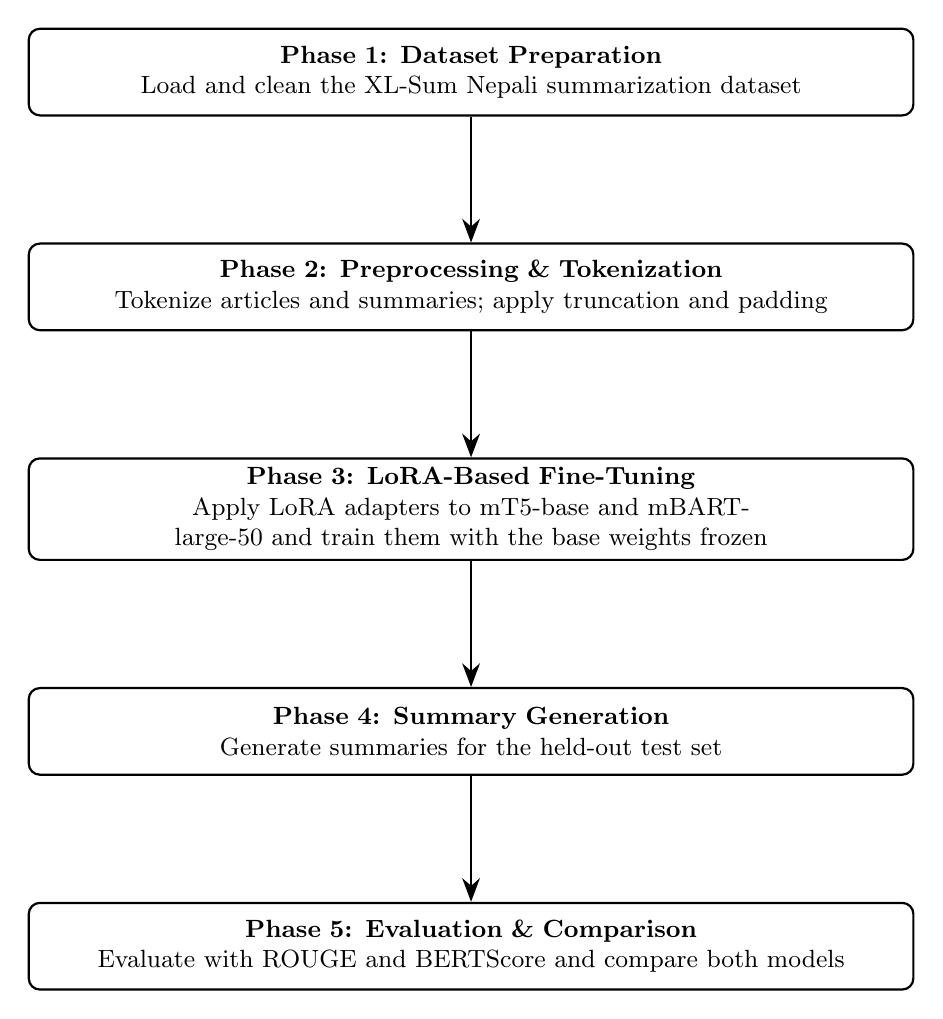
\begin{tikzpicture}[
    node distance=1.6cm,
    every node/.style={font=\small},
    phase/.style={
        rectangle,
        rounded corners,
        draw=black,
        thick,
        text width=11cm,
        align=center,
        minimum height=1.1cm
    },
    arrow/.style={
        -{Stealth[length=3mm]},
        thick
    }
]

\node (p1) [phase] {
\textbf{Phase 1: Dataset Preparation}\\
Load and clean the XL-Sum Nepali summarization dataset
};

\node (p2) [phase, below=of p1] {
\textbf{Phase 2: Preprocessing \& Tokenization}\\
Tokenize articles and summaries; apply truncation and padding
};

\node (p3) [phase, below=of p2] {
\textbf{Phase 3: LoRA-Based Fine-Tuning}\\
Apply LoRA adapters to mT5-base and mBART-large-50 and train them with the base weights frozen
};

\node (p4) [phase, below=of p3] {
\textbf{Phase 4: Summary Generation}\\
Generate summaries for the held-out test set
};

\node (p5) [phase, below=of p4] {
\textbf{Phase 5: Evaluation \& Comparison}\\
Evaluate with ROUGE and BERTScore and compare both models
};

\draw [arrow] (p1) -- (p2);
\draw [arrow] (p2) -- (p3);
\draw [arrow] (p3) -- (p4);
\draw [arrow] (p4) -- (p5);

\end{tikzpicture}

\caption{Research Methodology Flowchart}
\label{fig:research_flowchart}

\end{figure}

\subsection{Dataset}
The project uses the XL-Sum Nepali summarization dataset available on Hugging Face \cite{hasan2021xlsum}. Each sample consists of a Nepali news article (input) and a corresponding human-written abstractive summary (target). The dataset is divided into training, validation, and test splits, which are kept identical for both models.

\subsection{Data Preprocessing}
\begin{itemize}
    \item Load the Nepali summarization dataset.
    \item Remove invalid, empty, or missing samples.
    \item Tokenize articles and summaries using the tokenizer corresponding to each model (SentencePiece-based).
    \item Apply truncation and padding to fixed maximum input and target sequence lengths.
    \item Convert the processed data into tensors suitable for model training.
\end{itemize}

\subsection{LoRA-Based Fine-Tuning}
Both models are adapted using \textbf{parameter-efficient fine-tuning} with LoRA \cite{hu2021lora}. For each model the pretrained weights and tokenizer are loaded, LoRA adapters are attached to the attention layers, and the original pretrained parameters are frozen so that only the adapter parameters are trained. Each model is validated after every epoch and the best-performing adapters are saved for inference. During training:
\begin{itemize}
    \item Only the LoRA adapter parameters are updated through backpropagation, while the base model weights remain frozen.
    \item The cross-entropy loss between generated and reference summaries is minimized.
    \item Optimization uses the AdamW optimizer with an appropriate learning-rate scheduler.
    \item Validation performance is monitored after each epoch to select the best-performing checkpoint.
\end{itemize}

\subsection{Summary Generation}
After fine-tuning, summaries are generated for the test set. The generated token IDs are decoded back into readable Nepali text and compared against the corresponding human-written reference summaries.

\subsection{Implementation Tools}
\begin{itemize}
    \item \textbf{Programming Language:} Python
    \item \textbf{Deep Learning Framework:} PyTorch
    \item \textbf{Libraries:} Hugging Face Transformers, Hugging Face Datasets, PEFT (Parameter-Efficient Fine-Tuning), Evaluate, and SentencePiece
    \item \textbf{Development Environment:} Google Colab with GPU support
\end{itemize}


\chapter{Proposed Experimental Setup}
The experimental procedure applies the same dataset, preprocessing pipeline, and evaluation metrics to both models so that any difference in performance can be attributed to the models themselves.

\subsection{Experiment 1: LoRA-Adapted mT5-base}
\begin{itemize}
    \item Apply LoRA adapters to mT5-base and fine-tune them on the XL-Sum Nepali training set.
    \item Generate summaries for the test set.
    \item Evaluate the generated summaries using ROUGE and BERTScore.
\end{itemize}

\subsection{Experiment 2: LoRA-Adapted mBART-large-50}
\begin{itemize}
    \item Apply LoRA adapters to mBART-large-50 and fine-tune them on the same XL-Sum Nepali training set.
    \item Generate summaries for the same test set.
    \item Evaluate the generated summaries using ROUGE and BERTScore.
\end{itemize}

\subsection{Comparison and Analysis}
Finally, the ROUGE and BERTScore results of both models are compared, alongside training time and GPU memory usage. Differences in summary quality and generation behaviour are analysed to identify the model that performs best for Nepali abstractive summarization under LoRA-based fine-tuning. The experimental pipeline is summarized in Figure~\ref{fig:experiment_pipeline}.

\begin{figure}[htbp]
\centering

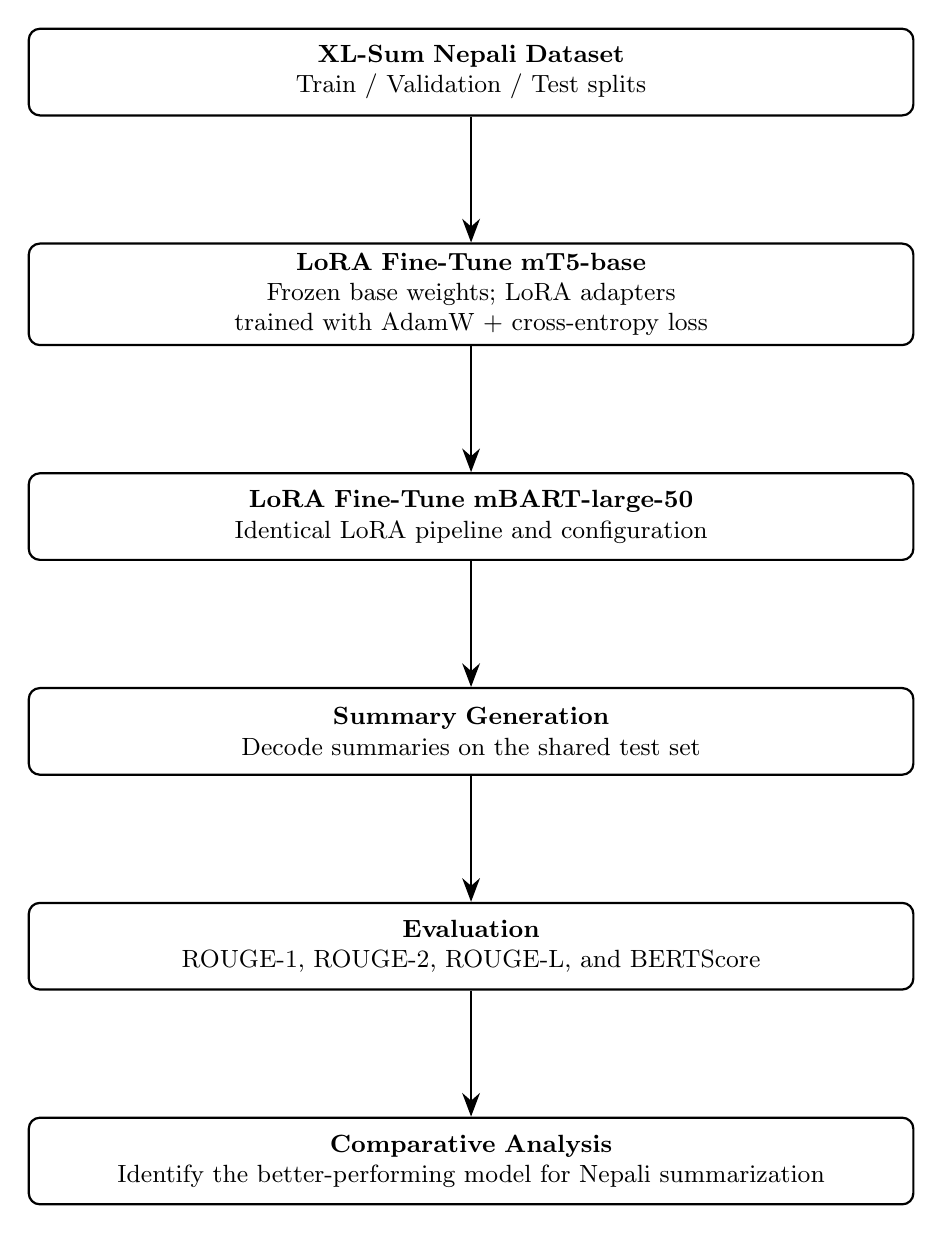
\begin{tikzpicture}[
node distance=1.6cm,
every node/.style={font=\small},
process/.style={
    rectangle,
    rounded corners,
    draw=black,
    thick,
    text width=11cm,
    align=center,
    minimum height=1.1cm
},
arrow/.style={
    -{Stealth[length=3mm]},
    thick
}
]

\node (data) [process] {
\textbf{XL-Sum Nepali Dataset}\\
Train / Validation / Test splits
};

\node (mt5) [process, below=of data] {
\textbf{LoRA Fine-Tune mT5-base}\\
Frozen base weights; LoRA adapters trained with AdamW + cross-entropy loss
};

\node (mbart) [process, below=of mt5] {
\textbf{LoRA Fine-Tune mBART-large-50}\\
Identical LoRA pipeline and configuration
};

\node (gen) [process, below=of mbart] {
\textbf{Summary Generation}\\
Decode summaries on the shared test set
};

\node (eval) [process, below=of gen] {
\textbf{Evaluation}\\
ROUGE-1, ROUGE-2, ROUGE-L, and BERTScore
};

\node (compare) [process, below=of eval] {
\textbf{Comparative Analysis}\\
Identify the better-performing model for Nepali summarization
};

\draw [arrow] (data) -- (mt5);
\draw [arrow] (mt5) -- (mbart);
\draw [arrow] (mbart) -- (gen);
\draw [arrow] (gen) -- (eval);
\draw [arrow] (eval) -- (compare);

\end{tikzpicture}

\caption{Experimental Pipeline for Comparing LoRA-Adapted mT5-base and mBART-large-50}
\label{fig:experiment_pipeline}
\end{figure}


\chapter{Expected Outcome}
This proposal is expected to deliver the following outcomes:
\begin{itemize}
    \item A LoRA-adapted mT5-base model for Nepali abstractive text summarization.
    \item A LoRA-adapted mBART-large-50 model for Nepali abstractive text summarization.
    \item A quantitative comparison of both models using ROUGE and BERTScore.
    \item Identification of the model that produces more accurate and semantically meaningful summaries for Nepali news articles while maintaining efficient resource utilization.
    \item A reproducible parameter-efficient fine-tuning pipeline for Nepali summarization.
\end{itemize}

It is anticipated that the larger mBART-large-50 may achieve higher lexical-overlap scores owing to its greater capacity, while mT5-base may offer competitive performance at a lower computational cost. Since both models are adapted with LoRA, the comparison also highlights how effectively parameter-efficient fine-tuning transfers each model to a low-resource language. The final comparison will clarify these trade-offs for practitioners working on Nepali summarization.


\chapter{Timeline}


\begin{figure}[ht]
    \centering
    \includegraphics[width=1\textwidth]{Screenshot 2026-07-03 at 16.31.15.png}
    \caption{Timeline chart}
    \label{fig:Timeline chart}

\end{figure}

\addcontentsline{toc}{section}{References}
\renewcommand{\bibname}{References}
\bibliographystyle{unsrt}
\bibliography{ref}

\end{document}

